\let\negmedspace\undefined
\let\negthickspace\undefined
\documentclass[journal]{IEEEtran}
\usepackage[a5paper, margin=10mm, onecolumn]{geometry}
\usepackage{tfrupee} 

\setlength{\headheight}{1cm}
\setlength{\headsep}{0mm}     

\usepackage{gvv-book}
\usepackage{gvv}
\usepackage{cite}
\usepackage{amsmath,amssymb,amsfonts,amsthm}
\usepackage{algorithmic}
\usepackage{graphicx}
\usepackage{textcomp}
\usepackage{xcolor}
\usepackage{txfonts}
\usepackage{listings}
\usepackage{enumitem}
\usepackage{mathtools}
\usepackage{gensymb}
\usepackage{comment}
\usepackage[breaklinks=true]{hyperref}
\usepackage{tkz-euclide} 
\usepackage{listings}
\def\inputGnumericTable{}                                 
\usepackage[latin1]{inputenc}                                
\usepackage{color}                                            
\usepackage{array}                                            
\usepackage{longtable}                                       
\usepackage{calc}                                             
\usepackage{multirow}                                         
\usepackage{hhline}                                           
\usepackage{ifthen}                                           
\usepackage{lscape}
\usepackage{circuitikz}


\tikzstyle{block} = [rectangle, draw, fill=blue!20, 
    text width=4em, text centered, rounded corners, minimum height=3em]
\tikzstyle{sum} = [draw, fill=blue!10, circle, minimum size=1cm, node distance=1.5cm]
\tikzstyle{input} = [coordinate]
\tikzstyle{output} = [coordinate]

\begin{document}

\bibliographystyle{IEEEtran}
\vspace{3cm}

\title{4.7.41}
\author{EE25BTECH11044 - Sai Hasini Pappula}
 \maketitle
{\let\newpage\relax\maketitle}

\renewcommand{\thefigure}{\theenumi}
\renewcommand{\thetable}{\theenumi}
\setlength{\intextsep}{10pt} 

\numberwithin{equation}{enumi}
\numberwithin{figure}{enumi}
\renewcommand{\thetable}{\theenumi}
\textbf{Question}

Find the distance of the point
\[
\vec{P}=\begin{bmatrix}2\\[2pt]4\\[2pt]-1\end{bmatrix}
\]

  from the line
\begin{equation}
\frac{x+5}{1}=\frac{y+3}{4}=\frac{z-6}{-9}.
\label{eq:given-line}
\end{equation}

\textbf{Solution}

\[
\text{Line: }\quad \vec r(t)=\vec a+t\vec m,\qquad
\vec a=\begin{bmatrix}-5\\[2pt]-3\\[2pt]6\end{bmatrix},\quad
\vec m=\begin{bmatrix}1\\[2pt]4\\[2pt]-9\end{bmatrix}.
\]

\subsection*{Derivation using the projection matrix}
For any nonzero vector \(\mathbf m\) the orthogonal projection matrix onto \(\mathbf m\) is
\begin{equation}
P=\frac{\mathbf m\mathbf m^{T}}{\mathbf m^{T}\mathbf m},
\end{equation}
so the component of a vector \(\mathbf v\) perpendicular to \(\mathbf m\) is \((I-P)\mathbf v\). Hence the distance from a point \(\mathbf p\) to the line through \(\mathbf a\) with direction \(\mathbf m\) is
\begin{equation}\label{eq:distance-matrix-derived}
d=\Big\lVert\Big(I-\frac{\mathbf m\mathbf m^{T}}{\mathbf m^{T}\mathbf m}\Big)(\mathbf p-\mathbf a)\Big\rVert.
\end{equation}

\subsection*{Equivalent scalar form}
Let \(\mathbf w=\mathbf p-\mathbf a\). Using \(P=\dfrac{\mathbf m\mathbf m^{T}}{\mathbf m^{T}\mathbf m}\) we get
\begin{equation}
d^{2}=\mathbf w^{T}(I-P)\mathbf w
= \mathbf w^{T}\mathbf w - \mathbf w^{T}\frac{\mathbf m\mathbf m^{T}}{\mathbf m^{T}\mathbf m}\mathbf w
= \lVert\mathbf w\rVert^{2} - \frac{(\mathbf m^{T}\mathbf w)^{2}}{\mathbf m^{T}\mathbf m}.
\end{equation}
This form is often quicker for computation.

\subsection*{Substitute the given vectors}
\begin{equation}
\mathbf p=\begin{bmatrix}2\\[2pt]4\\[2pt]-1\end{bmatrix},\qquad
\mathbf p-\mathbf a=\mathbf w=\begin{bmatrix}7\\[2pt]7\\[2pt]-7\end{bmatrix}.
\end{equation}
Compute the denominator:
\begin{equation}
\mathbf m^{T}\mathbf m = 1^{2}+4^{2}+(-9)^{2}=1+16+81=98.
\end{equation}
Compute the inner product \(\mathbf m^{T}\mathbf w\):
\begin{equation}
\mathbf m^{T}\mathbf w = 1\cdot 7 + 4\cdot 7 + (-9)\cdot(-7) = 7+28+63=98.
\end{equation}
Now use the scalar form:
\begin{equation}
\lVert\mathbf w\rVert^{2} = 7^{2}+7^{2}+(-7)^{2}=49+49+49=147,
\end{equation}
so
\begin{equation}
d^{2}=147-\frac{98^{2}}{98}=147-98=49
\end{equation}

\section*{Final Answer}
\[
\boxed{\,d=7\,}
\]

\begin{center}
    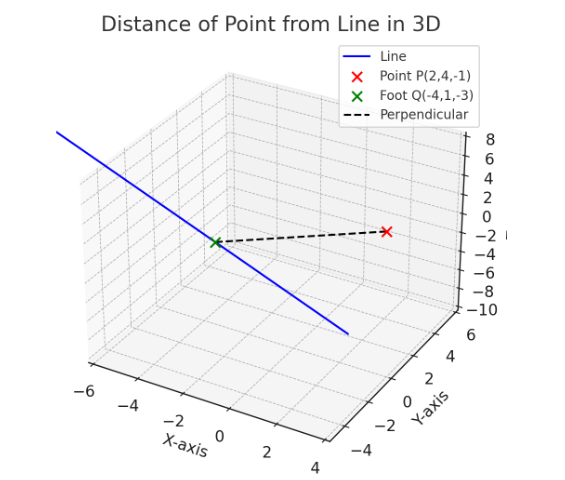
\includegraphics[width=0.8\columnwidth]{figs/plot7.png}
\end{center}

\end{document}